\subsection[]{MicroMegas}

\begin{frame}{MicroMegas (Micro-Mesh Gaseous Structure)}
    \begin{columns}[T]
	    \column{.5\textwidth}
			\begin{figure}[htbp]
			  \centering
			  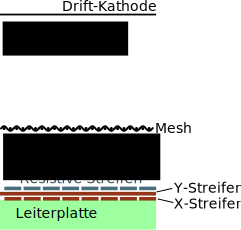
\includegraphics[width=\textwidth]{mm.jpg}
			  \caption{Aufbau MicroMegas}
			\end{figure}
			
	    \column{.55\textwidth}
	    	\begin{itemize}
	    	  \item flacher (großflächiger) Aufbau mit planarer Kathode und streifenförmiger Anode
	    	  \item Aufteilung der Kammer in zwei Bereiche: Driftbereich (ca 600~V/cm) und
	    	  Verstärkungsbereich (ca 50~kV/cm)
	    	  \item Bereiche getrennt durch Gitter (Mesh) $\rightarrow$ homogenes Feld zwischen Anode
	    	  und Mesh
	    	  \item Anode $\rightarrow$ resistive Streifen (Vermeidung Funken)
			\end{itemize}
			
    \end{columns}
\end{frame}


\begin{frame}{MicroMegas (Micro-Mesh Gaseous Structure)}
    \begin{columns}[T]
	    \column{.5\textwidth}
			\begin{figure}[htbp]
			  \centering
			  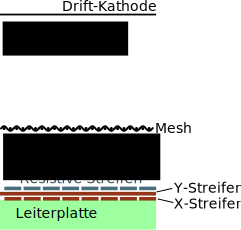
\includegraphics[width=\textwidth]{mm.jpg}
			  \caption{Aufbau MicroMegas}
			\end{figure}
			
	    \column{.55\textwidth}
	    	\begin{itemize}
	    	  \item eintreffende Teilchen erzeugen $e^-$/Ionen-Paare, die entlang Feldlinien Richtung
	    	  Mesh/Kathode driften
	    	  \item Mesh durchsichtig für freie $e^-$
	    	  \item Ladungslawinen im Verstärkungsbereich
	    	  \item Signalformung an Auslesedrähten über kapazitive Kopplung
			\end{itemize}
			
    \end{columns}
\end{frame}

\begin{frame}{MicroMegas}

	\begin{block}{Wie kommt die Spur zustande?}
		\begin{itemize}
		  \item zweidimensionale Ortsinformation durch zweilagige Auslesestreifen (senkrecht aufeinander)
		  \item mehrere Lagen hintereinander, um Spur zu rekonstruieren
		\end{itemize}
	\end{block}
	\vspace{0.8cm}
    \begin{columns}[T]
		\column{.45\textwidth}
			\bf{Vorteile}		
			\begin{itemize}
			  \item günstig
			  \item großflächiger Aufbau möglich
			  \item gute Ortsauflösung ($O(10\mu m)$)
			\end{itemize}	
	    \column{.5\textwidth}
	    	Nachteile
	    	\begin{itemize}
			  \item 
			\end{itemize}
    \end{columns}
    \vspace{1cm}
\end{frame}